\documentclass[12pt]{article} %Styl dokumentu
\usepackage{times} %Czcionka
\usepackage[a4paper,left=3.5cm,right=2.5cm,top=3cm,bottom=3cm,includefoot=false,includehead=false]{geometry} %Ustawienia marginesów
\linespread{1} %Interlinia
\setlength{\parindent}{0.5cm} %Wcięcie na początku akapitu
\setlength{\parskip}{1ex plus 0.5ex minus 0.2ex} %Odstępy pomiędzy akapitami

%Dodatkowe pakiety ******************************************************************
\usepackage[T1]{fontenc} %Styl tytułów rozdziałów
%\usepackage{subfig} NIE WIEM DO CZEGO ALE W PRZEJŚCIÓWCE TO MIAŁEM
%\usepackage{float} COS Z FLOATAMI ALE NIE WIEM CO, MOŻE NIE BĘDZIE NAM POTRZEBNE
\usepackage{amsfonts} %Niektóre symbole matematyczne
\usepackage{fixltx2e} %subscript
%\usepackage{pdfpages} %Dołączanie pdfów do tekstu
\usepackage{listings} %Pakiet od listingów programów
\usepackage{xcolor} %Pakiet kolorów do listingów programów Arduino
\usepackage{amsmath} %Pakiet matematyczny
\usepackage{bm,array} %Pakiet do tabel
\usepackage{fancyhdr} %Nagłówek i stopka
\usepackage{graphicx} %Wykresy i obrazy
\usepackage{subfigure} %Dodatkowa biblioteka do obrazów
\usepackage{polski} %Ustawienie języka polskiego
\usepackage[utf8]{inputenc} %Ustawienie kodowania polskich znaków
\usepackage{hyperref} %hiperłącza
\usepackage[labelfont=it,textfont={it}]{caption} %Formatowanie podpisów tabel i rysunków
\usepackage{wrapfig} %tekst obok rysunków
\usepackage{multirow}

%Definiowanie stylu Arduino dla listings*********************************************
\usepackage{xcolor}
\definecolor{stringColor}{rgb}{0.81,0.48,0}
\definecolor{kwordColor}{rgb}{0,0,0.90}
\definecolor{commentColor}{rgb}{0.59,0.59,0.59}
\definecolor{fieldColor}{rgb}{0,0.59,0}
\lstdefinelanguage{JavaL}{
      backgroundcolor=\color{white},  
      basicstyle=\footnotesize \ttfamily \color{black} \bfseries,   
      breakatwhitespace=false,       
      breaklines=true,               
      captionpos=b,                   
      commentstyle=\color{commentColor},   
      deletekeywords={...},          
      escapeinside={\%*}{*)},                  
      frame=single,                  
      language=Java,                
      keywordstyle=\color{kwordColor},  
      morekeywords={BRIEFDescriptorConfig,string,TiXmlNode,DetectorDescriptorConfigContainer,istringstream,cerr,exit}, 
      identifierstyle=\color{black},
      stringstyle=\color{stringColor},      
      numbers=left,                 
      numbersep=5pt,                  
      numberstyle=\color{black}, 
      rulecolor=\color{fieldColor},        
      showspaces=false,               
      showstringspaces=false,        
      showtabs=false,                
      stepnumber=1,                   
      tabsize=5,                     
      title=\lstname,                 
    }

%Nadpisywanie komend****************************************************************
\renewcommand{\theequation}{\thesubsection.\arabic{equation}}
\numberwithin{equation}{subsection}
\renewcommand{\thefigure}{\thesection.\arabic{figure}}
\renewcommand{\figurename}{Rys.} 
\numberwithin{figure}{section}
\renewcommand{\thetable}{\thesection.\arabic{table}}
\numberwithin{table}{section}
\renewcommand{\captionfont}{\small}
\renewcommand{\lstlisting}{\thesubsection.\arabic{lstlisting}}
\let\stdsection\subsection


\begin{document}

%---------------------------------------------------STRONA TYTUŁOWA-------------------------------------------------------------
\begin{center}
\end{center}
\vspace{1cm} 
\begin{center}
	\large{INSTYTUT AUTOMATYKI\\I INŻYNIERII INFORMATYCZNEJ\\WYDZIAŁ ELEKTRYCZNY\\POLITECHNIKA POZNAŃSKA\\}
\end{center}
\vspace{2cm} 
\begin{center}
	INŻYNIERSKA PRACA DYPLOMOWA\\
\end{center}
\begin{center}
	\Large{\textbf{SYSTEM WSPOMAGAJĄCY KIEROWANIE POJAZDEM\\Z UŻYCIEM ZŁĄCZA DIAGNOSTYCZNEGO}}
\end{center}
\begin{center}
	\large{\textbf{Mateusz BARTOSZ}}
\end{center}
\vspace{4cm}
\begin{flushright}
	Promotor:\\\textbf{Dr inż. Konrad URBAŃSKI}\\
\end{flushright}
\vspace{4cm} 
\begin{center}
	Poznań 2017
\end{center}

\thispagestyle{empty}
\newpage

%---------------------------------------------------POCZĄTEK DOKUMENTU-------------------------------------------------------------

\pagestyle{fancy}
\rhead{\thepage}
\lhead{\slshape \rightmark}
\lfoot{}
\cfoot{}
\rfoot{}

\tableofcontents
\thispagestyle{empty}

%---------------------------------------------------STRESZCZENIE-------------------------------------------------------------
\newpage
\thispagestyle{empty}
\section*{Streszczenie}
\vspace{0.5cm}
\hspace{0.5cm}W ramach niniejszej pracy zbudowany został układ umożliwiający komunikację ze złączem diagnostycznym OBD-II. Częściami układu są interfejs obsługujący połączenie z komputerem pokładowym samochodu oraz oprogramowanie umożliwiające pracę w trybie ręcznego wysyłania komend do interfejsu lub pracę w trybie automatycznym. Oprogramowanie składa się z dwóch współpracujących ze sobą modułów: interfejsu komunikacyjnego oraz graficznego interfejsu użytkownika. W ramach pracy omówiono strukturę zapytać wysyłanych do złącza diagnostycznego, otrzymywanych odpowiedzi, a także kodów błędów wysyłanych przez sterownik pojazdu. Dodatkowo zaprojektowano własny układ umożliwiający połączenie z pojazdami udostępniającymi do komunikacji linię K protokołu ISO 9141-2. Przeprowadzono również testy stworzonego oprogramowania i omówiono potencjalne zastosowania układu w realizacji zadań wspomagających prowadzenie pojazdu.
\newpage

\section*{Abstract}
\vspace{0.5cm}
\hspace{0.5cm}As part of this thesis system which enable coummunication with OBD-II connector was built. Parts of the system are the interface that supports connection to vehicle on-board computer and the software which allows to work in manual mode or automatic mode. The software consist of two cooperating modules: communication interface and graphical user interface. As part of disseration discusses the structure of requests sent to the diagnostic interface, receive responses and trouble code sent by the driver of the vehicle. In addition, own system for connecting to vehicles which provides communication via K-line ISO 9141-2 protocol was designed. Furthermote created software was tested in vehicle and potential applications of the system in the implementation of tasks to support driving was discussed. 


\thispagestyle{empty}
\vspace{0.5cm}
\hspace{0.5cm}

\newpage

%---------------------------------------------------WSTĘP-------------------------------------------------------------
\section{Wstęp}

	\subsection{Wybór tematu}
		\hspace{0.5cm}Głównym czynnikiem decydującym o wyborze tematu było zainteresowanie rozwiązaniami elektronicznymi stosowanymi we współczesnej motoryzacji oraz chęć podjęcia próby zbudowania układu opartego o własną koncepcję pracującego jako komputer pokładowy w samochodzie osobowym. Kolejnym czynnikiem było umożliwienie cyklicznego badania i kontroli parametrów pracy poszczególnych układów pojazdu, w celu uniknięcia lub wczesnego wykrycia potencjalnych usterek. Dodatkową motywacją była chęć zbudowania układu, który mógłby być w przyszłości praktycznie wykorzystywany w samochodach niewyposażonych w wbudowany komputer pokładowy. 	
	
	\subsection{Cel i zakres pracy}
		\hspace{0.5cm}Celem pracy było zaprojektowanie oraz wykonanie układu przyłącza do gniazda diagnostycznego w samochodzie osobowym Seat Cordoba II oraz zbudowanie interfejsu użytkownika umożliwiającego wizualizację odczytywanych parametrów, kontrolę wartości granicznych, a także przechowanie ich w celach dalszej diagnostyki. Dodatkowym celem było określenie możliwości wykorzystania odbieranych parametrów do opracowania algorytmów umożliwiających wspomaganie kierującego pojazdem, aby zoptymalizować jazdę, zwiększyć bezpieczeństwo podróży oraz zminimalizować ryzyko wystąpienia usterek. 
	
	\subsection{Założenia i wymagania}
		\hspace{0.5cm}Założeniem pracy jest opracowanie kompleksowego układu umożliwiającego odczytywanie, wizualizację oraz kontrolę parametrów odbieranych przez złącze diagnostyczne w samochodzie osobowym Seat Cordoba II, a także określenie możliwości wykorzystania tych parametrów do opracowania algorytmów wspomagających prowadzenie pojazdu.
	
		\newpage

%---------------------------------------------------ZAGADNIENIA WPROWADZAJĄCE-------------------------------------------------------------
\section{Zagadnienia wprowadzające}
	\hspace{0.5cm}We współczesnej motoryzacji wyraźnie można zauważyć tendencję automatyzacji procesu prowadzenia pojazdu oraz kontroli stanu jego parametrów. W samochodach dostępnych na rynku można spotkać bardzo wiele różnych protokołów komunikacyjnych. Cześć z nich służy do komunikacji pomiędzy urządzeniami wewnętrznymi pojazdu, inne do komunikacji z użytkownikiem, w celu zwiększenia komfortu jazdy, a jeszcze inne wykorzystywane są w diagnostyce stanu poszczególnych układów samochodu. Te ostatnie, wyprowadzone są do gniazda diagnostycznego(ang. On-Board Diagnosdic - OBD). W zależności od producenta, modelu oraz roku produkcji pojazdu do dyspozycji są różne protokoły. Umożliwiają one między innymi odczytywanie aktualnych wskazań niektórych czujników, kontrolę zużywania się elementów eksploatacyjnych czy detekcję błędów silnika. W niniejszym rozdziale omówione zostało złącze diagnostyczne w wersji drugiej(ODB2) wraz z udostępnianymi przez nie protokołami komunikacyjnymi.

	\subsection{Złącze diagnostyczne}
		\hspace{0.5cm}Historia złącza diagnostycznego używanego w motoryzacji sięga końcówki lat sześćdziesiątych dwudziestego wieku. Pierwsze komputery pokładowe wprowadzone zostały w samochodach marki Volkswagen w 1968 roku. Dziesięć lat później za sprawą marki Nissan komputery pokładowe pojawiły się w pojazdach konsumenckich. Kolejnym krokiem było wprowadzenie protokołu ALDL  przez General Motors w 1980 roku. Był to pierwszy standard zbliżony do obecnie stosowanego w gniazdach OBD2. Występował w trzech wersjach: dwunasto, dziesięcio i pięciopinowej. Pierwsze wersje były jednokierunkowe i umożliwiały przesyłanie 160 bodów danych. W późniejszych wersjach wprowadzono dwukierunkową transmisję danych o zwiększono szybkości transmisji do 8192 bodów. W 1991 roku agencja California Air Resources Board zażądała, aby każdy nowy pojazd sprzedawany w Kalifornii posiadał wyprowadzenie diagnostyczne. Stało się to impulsem do opracowania i wprowadzenia standardu OBD-I, choć nazwa ta została wprowadzona dopiero po opracowaniu kolejnego standardu OBD w wersji drugiej. Złącze ODB-I nie zostało ściśle ustandaryzowane i każdy producent samochodów mógł wykonać je w swojej wersji. Główną motywacją do wprowadzenia tego standardu było zachęcenie producentów pojazdów do zaprojektowania systemów kontroli emisji spalin. Często spotykana wersja tego złącza umożliwiała odczytywanie kodów błędów poprzez analizę migania diody znajdującej się przy złączu. Miganie diody reprezentowało odpowiednią liczbę dwucyfrową, która była interpretowana jako odpowiedni kod błędu pojazdu. W 1994 roku na bazie poprawionej i uzupełnionej specyfikacji OBD-I powstał standard ODB-II. Jest to najpopularniejszy, aktualnie używany system diagnostyki samochodowej. Od roku 1996 wszystkie nowe samochody sprzedawane w Stanach Zjednoczonych muszą być wyposażone właśnie w gniazdo ODB w wersji drugiej. W 2001 roku standard OBD-II pod nazwą EOBD został wprowadzony jako obowiązkowy w samochodach benzynowych produkowanych w Unii Europejskiej, a w 2003 roku również w samochodach z silnikami wysokoprężnymi.
		
		\newpage
		
		\subsubsection{Złącze diagnostyczne OBD-II}
			\hspace{0.5cm}Złącze diagnostyczne OBD w wersji drugiej jest aktualnie stosowanym w motoryzacji wyprowadzeniem umożliwiającym wykrywanie błędów poszczególnych układów pojazdu. Opis budowy tego złącza zawarty jest w normie SAE J1962[\cite{saej1962}]. Standard OBD-II zawiera specyfikację dotyczącą budowy złącza, a także opis udostępnianych przez nie protokołów komunikacyjnych. Zgodnie z normą, złącze występuje w dwóch wersjach: A oraz B, oba szesnastopinowe (2x8), żeńskie. Na Rys. \ref{rys_obd2_wtyczka} przedstawiono budowę obu typów złączy.
		
		\begin{figure}[ht]
		\centering
		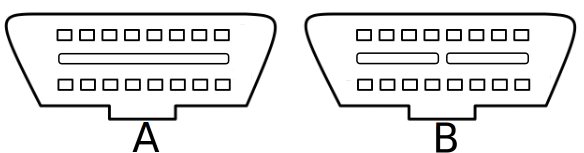
\includegraphics[scale=0.8]{Images/ZlaczaOBD2.pdf}
		\caption{Porównanie złącza diagnostycznego w wersji A oraz B.}
		\label{rys_obd2_wtyczka}
		\end{figure}
		
		Złącze typu A stosowane jest w pojazdach wyposażonych w akumulator o napięciu 12V, natomiast złącze typu B w pojazdach wyposażonych w akumulator o napięciu 24V.
		
		Norma SAE J1962 definiuje protokoły komunikacyjne udostępniane przez złącze diagnostyczne. Dostępność poszczególnych protokołów komunikacyjnych może być różna w zależności od producenta pojazdu oraz roku produkcji. Na Rys. \ref{rys_obd2_pinout} oraz w tabeli \ref{tab_obd2_pinout} przedstawione zostały potencjalnie dostępne protokoły komunikacyjne wraz z numerem pinu, do którego powinny być podłączone.
		
		\begin{figure}[ht]
		\centering
		\includegraphics[scale=0.8]{Images/ZlaczeOBD2_pinout.pdf}
		\caption{Opis wyprowadzeń złącza diagnostycznego. Wykorzystywane wyprowadzenia zostały zaznaczone kolorem niebieskim oraz odpowiednim numerem. Opis wyprowadzeń znajduje się w Tab \ref{tab_obd2_pinout}}
		\label{rys_obd2_pinout}
		\end{figure}
		
		W złączu diagnostycznym udostępnionych jest 5 różnych protokołów. Dodatkowo rozróżnione są dwie masy: masa podwozia oraz masa sygnałowa. W praktyce najczęściej wyprowadzenia te są ze sobą zwarte. Zazwyczaj w pojazdach udostępniony jest tylko jeden z opisanych poniżej protokołów. 
		
		\newpage
		
		\begin{table}[ht]
\centering
\caption{Opis wyprowadzeń złącza diagnostycznego OBD-II.}
\label{tab_obd2_pinout}
\begin{tabular}{|c|c|}
\hline
\textbf{Numer wyprowadzenia} & \textbf{Przeznaczenie wyprowadzenia}                                                                    \\ \hline
2                            & Linia dodatnia protokołu SAE J1850 PWM oraz VPW                                                         \\ \hline
4                            & Masa podwozia                                                                                           \\ \hline
5                            & Masa sygnałowa                                                                                          \\ \hline
6                            & Linia wysoka magistrali CAN                                                                             \\ \hline
7                            & Linia K protokołu ISO 9141-2 oraz ISO 14230-4                                                           \\ \hline
10                           & Linia ujemna protokołu SAE J1850 PWM                                                                    \\ \hline
14                           & Linia niska magistrali CAN                                                                              \\ \hline
15                           & Linia L protokołu ISO 9141-2 oraz ISO 14230-4                                                           \\ \hline
16                           & \begin{tabular}[c]{@{}c@{}}Zasilanie\\ 12V/4A dla złącza typu A\\ 24V/2A dla złącza typu B\end{tabular} \\ \hline
\end{tabular}
\end{table}

		\subsubsection{Protokoły komunikacyjne dostępne w złączu diagnostycznym}
		\hspace{0.5cm}Zgodnie z normą SAE J1962 do złącza diagnostycznego doprowadzone może być pięć różnych magistral danych które udostępniają następujące protokoły komunikacji:
		
		\begin{itemize}
			\item{SAE J1850 PWM,}
			\item{SAE J1850 VPW,}
			\item{CAN,}
			\item{ISO 9141,}
			\item{ISO 14230 - KWP2000.}
		\end{itemize}
		
		SAE  J1850 to  magistrala wykorzystywana głównie w samochodach marek amerykańskich. Występuje w dwóch odmianach. Pierwsza z nich to J1850 PWM (Pulse width modulation). Jest to technologia komunikacji wykorzystująca modulację szerokością impulsu do kodowania logicznych stanów (0 oraz 1). Każdy bit zaczyna się zmianą stanu niskiego na wysoki. Następnie, w zależności od wysyłanego bitu danych, zmienia się wypełnienie impulsu, dla logicznego „0” stan wysoki utrzymuje się przez 2/3 czasu impulsu, natomiast dla „1” stan wysoki to 1/3 impulsu. Czas trwania impulsu jest stały. Magistrala jest dwuprzewodowa, kodowanie różnicą pomiędzy potencjałami obu kanałów. Prędkość transmisji wynosi 41,6 kb/s. Głównym koncernem wykorzystującym magistralę J1850 PWM jest Ford.
		
		\newpage
		
		Drugą odmianą magistrali J1850 jest wersja VPW (variable pulse width). W tej wersji każdy nowy bit sygnalizowany jest za pomocą zmianą stanu. W związku z tym, aby rozpoznać logiczne zmiany, w zależności od wartości poprzedniego bitu kolejny bit kodowany jest za pomocą długości impulsu, nie zaś stanem wysokim lub niskim.  W związku z tym, że długości bitów są różne,  nie można jednoznacznie określić prędkości transmisji, przyjmowane jest średnio 10,4 kbit/s. Jest to magistrala jednoprzewodowa, używana przez General Motors.
		
		Magistrala CAN (Controller Area Network), zastosowana pierwszy raz przez koncern Mercedes w roku 1992,  umożliwia komunikację pomiędzy urządzeniami oraz mikrokontrolerami bez używania urządzenia nadrzędnego.  Początkowo używany w branży motoryzacyjnej, został również z powodzeniem wprowadzony do automatyki przemysłowej. Transmisja sygnału odbywa się za pomocą dwóch przewodów, na każdym występują dwa stany. Jeden stan jest zgodny (dla linii wysokiej oraz niskiej potencjał jest ten sam), oznacza logiczne 0, drugi stan sygnalizowany jest za pomocą wysokiego stanu na linii „High”, a niskim na linii „Low”. 
		
		Tańszym odpowiednikiem CAN stosowanym we wcześniejszych pojazdach jest magistrala oparta na normie ISO 9141,  LIN (Local Interconnect Network).  Komunikacja opiera się na architekturze master/slave. Komunikacja wywoływana jest poprzez zapytanie wysyłane przez mastera, przez co nie ma konieczności wykrywania kolizji. Jest to sieć stworzona jednoprzewodowo lub dwuprzewodowo, w zależności od zastosowania, pozwalająca na podłączenie maksymalnie 16 urządzeń do jednej sieci. Maksymalna prędkość przesyłania to 20 kbit/s.
		
		\newpage
		
		\subsection{Struktura zapytań złącza diagnostycznego}
		
		\hspace{0.5cm}Głównym zastosowaniem złącza diagnostycznego miało być nadzorowanie systemów, które mają znaczenie w emisji spalin. Specyfikacja na temat transmisji danych diagnostycznych dostępne są w normie ISO 15031 oraz bliźniaczej SAE J1979. Jako systemy podległe normy dopuszczają sieć K-Line z KWP 200 oraz jej poprzednika ISO 9141-2 CARB, KWP 2000 z CAN oraz stosowaną głównie w pojazdach amerykańskich producentów magistralę SAE J1850 w wersji VPW i PWM.
		
		Komunikacja z OBD odbywa się w postaci żądanie - odpowiedź(and request - response) i ma formę protokołu KWP 2000 \cite{Schmidgall08}. Komunikat żądania podzielony jest na trzy części. Pierwszą z nich stanowi identyfikator serwisu (ang. Service ID - SID), który w normie amerykańskiej nazywane jest trybem testowym lub po prostu trybem (ang. test modes). Tryby o numerach 01-09 są nazywane trybami podstawowymi, natomiast tryby powyżej numeru 09 trybami rozszerzonymi\cite{Merkisz02}. W tabeli \ref{tab_pid_modes} przedstawione zostały dostępne podstawowe identyfikatory serwisu.
		
		\begin{table}[ht]
\centering
\caption{Tryby pracy złącza diagnostycznego\cite{Schmidgall08}.}
\label{tab_pid_modes}
\begin{tabular}{|c|l|}
\hline                                                                 
\textbf{SID (hex)} & \multicolumn{1}{c|}{\textbf{Opis}}                                                                                                                                      \\ \hline
01                 & \begin{tabular}[c]{@{}l@{}}Pytania o wartości danych w sterowniku. Dane są \\ identyfikowane za pomocą kodu PID\end{tabular}                                            \\ \hline
02                 & \begin{tabular}[c]{@{}l@{}}Pytanie o dane dotyczące warunków otoczenia dla kodów \\ usterek zapisanych w pamięci.\end{tabular}                                          \\ \hline
03                 & \begin{tabular}[c]{@{}l@{}}Odczytywanie z pamięci błędów mających wpływ na emisję\\  spalin zakwalifikowanych jako ,,wykryte bezzasadnie''.\end{tabular}                \\ \hline
04                 & \begin{tabular}[c]{@{}l@{}}Kasowanie pamięci błędów (kodów błędów, warunków\\ otoczenia, statusu różnych testów)\end{tabular}                                           \\ \hline
05                 & Nadzorowanie sondy lambda                                                                                                                                               \\ \hline
06                 & \begin{tabular}[c]{@{}l@{}}Nadzorowanie katalizatorów, układów wylotowych,\\ ogrzewania sondy lambda i katalizatorów,  układów\\ wtrysku paliwa i zapłonu.\end{tabular} \\ \hline
07                 & \begin{tabular}[c]{@{}l@{}}Podobnie jak dla SID=03, tutaj są odsyłane tylko błędy, \\ które zostały zakwalifikowane jako ,,wykryte przejściowo''.\end{tabular}          \\ \hline
08                 & Test poziomu paliwa                                                                                                                                                     \\ \hline
09                 & Wyświetlanie informacji o pojeździe      \\ \hline  
\end{tabular}
\end{table}

Opis trybów rozszerzonych można znaleźć w literaturze \cite{Merkisz02}.
	
	Kolejną częścią wysyłanego żądania jest identyfikator parametru - PID (ang. Parameter Identifier). Zajmuje on również 1 bajt oraz kodowany jest szesnastkowo. Ostatnią częścią zapytania są parametry żądania, które mogą zająć maksymalnie 6 bajtów. Najczęściej jednak wykorzystuje się żądania bez dodatkowych parametrów.

	\newpage

	W złączu diagnostycznym pojazdu nie muszą być udostępnione wszystkie tryby pracy, a także nie muszą być udostępnione wszystkie kody zapytań z udostępnionego trybu. Ogólna struktura kodów zapytań ma postać:

	\begin{itemize}
		\item{AA BB CC CC CC CC CC,}
	\end{itemize}
		 gdzie AA to numer trybu testowego , BB to identyfikator z wybranego trybu natomiast CC dodatkowe parametry. Kody BB oraz CC są opcjonalne, natomiast kod AA musi być zawarty w każdym zapytaniu. 
		 
		 Struktura odpowiedzi złącza diagnostycznego na zadany kod jest podobna do zapytania. Pierwszy bajt to kod SID zapytania, ale po wykonaniu (AA|40), czyli po dodaniu do kodu SID zapytania liczby 40 kodowanej szesnastkowo. Drugi bajt jest powtórzeniem identyfikatora parametru żądania. Następnie w odpowiedź może się znaleźć do sześciu bajtów parametrów odpowiedzi. Ogólna struktura kodów odpowiedzi ma zatem postać:
		
		\begin{itemize}
			\item{AA|40 BB CC CC CC CC CC.}
		\end{itemize}		
		 
		 Ilość odebranych danych, a także ich interpretacja jest różna w zależności od identyfikatora parametru. Strukturę oraz interpretację odpowiedzi można przeanalizować na przykładzie. Wysyłając do złącza diagnostycznego żądanie 01 00 w odpowiedzi zwrócona zostanie informacja o udostępnionych identyfikatora parametru trybu 01 z zakresu 01-20:
		
		\begin{itemize}
			\item{01 00}
			\item{41 00 BE 1F B8 10}
		\end{itemize}
		
		Odpowiedź - po usunięciu z niej nagłówka - należy zapisać w postaci binarnej, w której wartość 1 oznacza że dany kod jest udostępniony. Sposób dekodowanie odpowiedzi przedstawiony zostały w tabeli \ref{tab_pid_response}
		
\begin{table}[!h]
\centering
\caption{Interpretacja odpowiedzi na kod zapytania 01 00}
\label{tab_pid_response}
\begin{tabular}{|c|c|c|c|c|c|c|c|c|c|c|}
\hline
\textbf{\begin{tabular}[c]{@{}c@{}}Bajt\\ odpowiedzi\\ (hex)\end{tabular}} & \multicolumn{4}{c|}{B} & \multicolumn{4}{c|}{E} & \textbf{.} & \textbf{.} \\ \hline
\textbf{\begin{tabular}[c]{@{}c@{}}Postać\\ binarna\end{tabular}}          & 1    & 0   & 1   & 1   & 1    & 1   & 1   & 0   & \textbf{.} & \textbf{.} \\ \hline
\textbf{Kod PID}                                                           & 01   & 02  & 03  & 04  & 05   & 06  & 07  & 08  & \textbf{.} & \textbf{.} \\ \hline
\end{tabular}
\end{table}		
		
		Wartości identyfikatora parametru powtarzające się co wartość 20 w kodzie szesnastkowym(00, 20, 40) zarezerwowane są do odczytywania udostępnionych przez dany sterownik kodów PID i dekoduje się je zawsze tak jak przedstawiono w przykładzie.
		\newpage
		
		Najczęściej jednak żadnie dotyczy konkretnego parametru pojazdu. Odpowiedź otrzymana na żądanie jest wtedy dekodowana na podstawie wzoru:
		
	\begin{equation}
	x_{fiz} = (x_{hex}) \times {(2^n-1)}^{-1} \times (V_{max} - V_{min}) + V_{min},
	\end{equation}			
	gdzie: $x_{fiz}$ - obliczona wartość fizyczna, $x_{hex}$ - odebrana wartość w postaci szesnastkowej, n - liczba bitów odpowiedzi, $V_{max}$ - wartość maksymalna zakresu zmiennej, $V_{min}$ - wartość minimalna zakresu zmiennej.
		
		\newpage
		
		\subsection{Struktura kodów błędów}
		
		\hspace{0.5cm}Podstawową funkcjonalnością złącza diagnostycznego jest raportowanie błędów poszczególnych układów za pomocą diagnostycznych kodów błędów(ang. Diagnostic Trouble Codes - DTC). Są one zapisywane w sterowniku jako 16-bitowe liczby heksadecymalne, a następnie przetwarzane przez tester diagnostyczny to postaci 5-znakowego słowa alfanumerycznego. Aby uzyskać informację o zapisanych kodach należy wysłać zapytanie 03 do złącza diagnostycznego, ale najpierw zdefiniować ile kodów jest obecnych w pamięci. W tym celu należy wysłać komendę:
		
		\begin{itemize}
			\item{01 01.}
		\end{itemize}
		Kod odpowiedzi powinien mieć postać zbliżoną do: 

		\begin{itemize}
			\item{41 01 81 07 65 04.}
		\end{itemize}
		
		Wartości 41 01 to nagłówek odpowiedzi. Właściwa odpowiedź zaczyna się od dwóch pary bajtów 81, w których zapisana jest informacja o ilości przechowywanych kodów błędów pojazdu. Wartość 81 to liczba zapisana w postaci szesnastkowej, której wartość w systemie dziesiętnym to 129. Nie jest to jednak wprost liczba kodów błędów. W kodzie tym zawarta jest również informacja o stanie diody kontrolnej silnika, który zapisany jest na najbardziej znaczącym bicie, co oznacza, że odczytaną wartość należy pomniejszyć o 128 lub 80 w systemie szesnastkowym. Wynika z tego że w zaprezentowanym przykładzie przechowywany jest tylko jeden kod błędu. Podany przykład ilustruję sytuację, w której pojazd udostępnia tylko jeden moduł, który raportuje kody błędów. Jeżeli takich modułów byłoby więcej w odpowiedzi na instrukcję 01 01 wysłana zostanie odpowiedź podobna do przedstawionej dla każdego modułu. W celu sprawdzenia z którego modułu wysłana została odpowiedź należy włączyć wysyłanie nagłówka odpowiedzi.
		
		Po ustaleniu liczby przechowywanych błędów można przejść do odczytywania ich kodów poprzez wysłanie instrukcji 03. Odpowiedź powinna mieć postać zbliżoną do:
		
		\begin{itemize}
			\item{43 01 33 00 00 00 00.}
		\end{itemize}
		
		Wartość 43 to nagłówek odpowiedzi na kod 03. Kolejnych 6 bajtów powinno być odczytywanych parami. Każda para reprezentuje jeden kod błędu. W powyższym przypadku przechowywany jest tylko jeden kod 0133, natomiast zgodnie z standardem SAE odpowiedź została uzupełniona bajtami 00, które nie są interpretowane jako kody diagnostyczne. Pierwsza cyfra w odczytanym kodzie zawsze przechowuje zakodowaną informację o źródle błędu. Sposób dekodowania źródła wystąpienia błędu przedstawiony został w tabeli \ref{tab_dtc_interpret}.
		
		\newpage
		
		\begin{table}[!h]
\centering
\caption{Kodowanie źródła błędu \cite{White06}.}
\label{tab_dtc_interpret}
\begin{tabular}{|c|c|l|}
\hline
\textbf{\begin{tabular}[c]{@{}c@{}}Pierwsza cyfra\\ odpowiedzi\end{tabular}} & \textbf{\begin{tabular}[c]{@{}c@{}}Zakodowany\\ identyfikator\end{tabular}} & \multicolumn{1}{c|}{\textbf{Opis}} \\ \hline
0                                                                            & P0                                                                          & \begin{tabular}[l]{@{}l@{}}Kody układu napędowego\\ zdefiniowane w normie SAE\end{tabular} \\ \hline
1                                                                            & P1                                                                          & \begin{tabular}[l]{@{}l@{}}Kody zdefiniowane\\ przez producenta\end{tabular}                \\ \hline
2                                                                            & P2                                                                          & \begin{tabular}[l]{@{}l@{}}Kody zdefiniowane\\ w normie SAE\end{tabular}                    \\ \hline
3                                                                            & P3                                                                          & \begin{tabular}[l]{@{}l@{}}Kody zdefiniowane\\ przez producenta\end{tabular}                \\ \hline
4                                                                            & C0                                                                          & \begin{tabular}[l]{@{}l@{}}Kody podwozia zdefiniowane\\ w normie SAE\end{tabular}           \\ \hline
5                                                                            & C1                                                                          & \begin{tabular}[l]{@{}l@{}}Kody zdefiniowane\\ przez producenta\end{tabular}                \\ \hline
6                                                                            & C2                                                                          & \begin{tabular}[l]{@{}l@{}}Kody zdefiniowane\\ przez producenta\end{tabular}                \\ \hline
7                                                                            & C3                                                                          & \begin{tabular}[l]{@{}l@{}}Kody zdefiniowane\\ w normie SAE\end{tabular}           \\ \hline
8                                                                            & B0                                                                          & \begin{tabular}[l]{@{}l@{}}Kody nadwozia zdefiniowane \\ w normie SAE\end{tabular}                   \\ \hline
9                                                                            & B1                                                                          & \begin{tabular}[l]{@{}l@{}}Kody zdefiniowane \\ przez producenta\end{tabular}               \\ \hline
A                                                                            & B2                                                                          & \begin{tabular}[l]{@{}l@{}}Kody zdefiniowane \\ przez producenta\end{tabular}               \\ \hline
B                                                                            & B3                                                                          & \begin{tabular}[l]{@{}l@{}}Kody zdefiniowane\\ w normie SAE\end{tabular}          \\ \hline
C                                                                            & U0                                                                          & \begin{tabular}[l]{@{}l@{}}Kody sieci zdefiniowane \\ w normie SAE\end{tabular}             \\ \hline
D                                                                            & U1                                                                          & \begin{tabular}[l]{@{}l@{}}Kody zdefiniowane \\ przez producenta\end{tabular}               \\ \hline
E                                                                            & U2                                                                          & \begin{tabular}[l]{@{}l@{}}Kody zdefiniowane \\ przez producenta\end{tabular}               \\ \hline
F                                                                            & U3                                                                          & \begin{tabular}[l]{@{}l@{}}Kody zdefiniowane\\ w normie SAE\end{tabular}          \\ \hline
\end{tabular}
\end{table}
		
	Kod błędu z przykładowej odpowiedzi to 0133. Pierwszą cyfrę należy zastąpić wartością z tabeli, a pozostałe trzy cyfry pozostawić bez zmiany. W przedstawionym przykładzie daje to wartość P0133 co oznacza wystąpienie błędu wolnej odpowiedzi obwodu czujnika tlenu. Analogicznie po otrzymaniu odpowiedzi w postaci D016 odczytanym kodem jest U1016. Znaczenie wszystkich kodów błędów można odnaleźć w dokumentacji normie \cite{saej1979} lub w literaturze \cite{White06}.
	
	
	\newpage	
	
	\subsection{Interfejs komunikacyjny ELM 327}\label{rozdzial_elm}
	
	\hspace{0.5cm}Do komunikacji ze złączem diagnostyczny można wykorzystać popularny interfejs ELM327 firmy ELM Electronics. Dostępny jest w dwóch wariantach: RS232 lub bluetooth. Jądrem urządzenia jest mikroprocesor PIC18F2480 firmy Microchip Technology. W niniejszej pracy wykorzystany zostało urządzenie udostępniające komunikację bluetooth pokazane na Rys. \ref{rys_elm327}.
	
	\begin{figure}[ht]
		\centering
		\includegraphics[scale=1]{Images/rys_elm327.png}
		\caption{ELM 327 w wersji bluetooth.}
		\label{rys_elm327}
		\end{figure}
	
	Interfejs ELM327 umożliwia współpracę ze wszystkimi udostępnionymi w złączu diagnostycznym protokołami. Komunikacja modułu z komputerem odbywa się poprzez wirtualny port szeregowy. W celu umożliwienia poprawnej komunikacji należy skonfigurować port zgodnie z następującymi parametrami:
	
	\begin{itemize}
		\item{prędkość transmisji : 15200 bit/s,}
		\item{liczba bitów danych : 8,}
		\item{parzystość : żaden,}
		\item{liczba bitów stopu : 1.}
	\end{itemize}	
	
	Z modułem można się komunikować za pomocą komend AT zdefiniowanych w dokumentacji producenta \cite{elm327}. Żeby żądanie zostało wysłane do interfejsu każdą instrukcję należy zakończyć znakiem powrotu karetki. Przykładowa komenda z odpowiedzią do wyłączania echa instrukcji w odpowiedzi wraz ma następującą postać:
	
	\begin{itemize}
		\item{ATE0}
		\item{ATE0OK}
	\end{itemize}	
	
	\newpage
	
%---------------------------------------------------STRUKTURA PROJEKTU-------------------------------------------------------------	
	\section{Struktura projektu}
	\hspace{0.5cm}Zrealizowany projekt układu do komunikacji ze złączem diagnostycznym składa się z trzech głównych modułów:
	
	\begin{itemize}
		\item{Moduł komunikacji ze złączem diagnostycznym}
		\item{Oprogramowanie umożliwiające komunikację z komputera z wymienionym wyżej modułem oraz zapisywanie danych pomiarowych}
		\item{Oprogramowanie wizualizujące odczytane parametry}
	\end{itemize}
	
	Struktura zbudowanego układu przedstawiona jest na Rys. \ref{rys_schemat_ukladu}.
	
		\begin{figure}[ht]
		\centering
		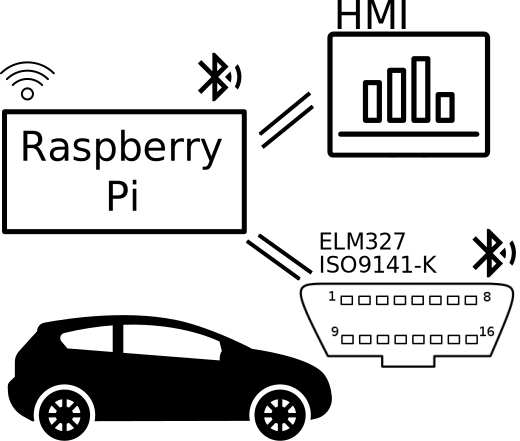
\includegraphics[scale=0.8]{Images/SchematUkladu.pdf}
		\caption{Schemat układu. Opis w tekście.}
		\label{rys_schemat_ukladu}
		\end{figure}
	
	W pierwszej fazie projektu planowano wykonać autorski moduł do komunikacji ze złączem diagnostycznym. W tym celu zaprojektowany został układ oparty o mikroprocesor STM32F103CBT6 opisany w rozdziale \ref{rozdzial_uklad_stm}. Niestety ze względu na zbyt wysoką cenę wykonania tylko jednej sztuki prace zakończono na projekcie schematu elektrycznego oraz obwodu drukowanego. Jako zamiennik autorskiego układu w pracy wykorzystano popularne urządzenie ELM327 v2.1 udostępniające komunikację bezprzewodową bluetooth. 
	
	\newpage
	
	Jako moduł główny w projekcie zdecydowano się wykorzystać komputer \mbox{Raspberry Pi 3} ze względu na jego dobry stosunek jakości do ceny. Przy wyborze tego układu ważna również była możliwość podłączenia zewnętrznego ekranu, a także dostępność komunikacji bluetooth. Oprogramowanie obsługujące funkcjonalność napisane zostało w języku Java SE 8 z wykorzystaniem dodatkowej biblioteki pi4j umożliwiającej dostęp dostęp do funkcji wbudowanych komputera Raspberry Pi, takich jak komunikacja bluetooth, czy zarządzanie portami GPIO. Dodatkowo oprogramowanie wykorzystuje bibliotekę jbidibc-rxtx-2.2 umożliwiającą wykorzystanie portów szeregowych komputera, które były niezbędne do komunikacji z urządzeniem ELM327. Dokładny opis funkcjonalności stworzonego oprogramowania znajduje się w rozdziale \ref{rozdzial_raspberry_software}.
	
	Ostatni moduł - interfejs graficzny użytkownika - stworzony został w języku \mbox{Java SE 8} z wykorzystaniem nowego frameworku do tworzenia zaawansowanych interfejsów graficznych JavaFX 8. Interfejs użytkownika dostosowany został do wykorzystywania na urządzeniach wyposażonych w ekran dotykowy o rozdzielczości 1024x600 pikseli. Do umożliwienia zapisywania danych w celu sporządzania dalszych statystyk stworzona została relacyjna baza danych wykorzystująca darmowy serwer MySQL Community Server w wersji 5.7 firmy Oracle. Dokładny opis funkcjonalności stworzonego oprogramowania wraz z przykładowymi widokami panelu użytkownika znajduje się w rozdziale \ref{rozdzial_hmi_software}. Poszczególne elementy układu przedstawione zostały na Rys. \ref{rys_uklad_widok}.
	
	\begin{figure}[!h]
		\centering
		\includegraphics[scale=0.14]{Images/rys_uklad_widok.png}
		\caption{Poszczególne elementy układu.}
		\label{rys_uklad_widok}
		\end{figure}
	
	\newpage	
	
%---------------------------------------------------PROJEKT PŁYTKI-------------------------------------------------------------	
\section{Projekt układu do komunikacji ze złączem diagnostycznym} \label{rozdzial_uklad_stm}
	
	\hspace{0.5cm}W ramach pracy planowano wykonać interfejs komunikacyjny umożliwiający połączenie komputera pokładowego pojazdu z komputerem Raspberry Pi. Ze względów finansowych ostatecznie zaniechano wykonania modułu, a prace zakończono na etapie projektu, którego opis przedstawiony został w niniejszym rozdziale. Jako zamiennik własnego układu zastosowano popularny moduł ELM 327, którego opis znajduje się w rozdziale \ref{rozdzial_elm}.
	
	Schemat ideowy zaprojektowanego interfejsu komunikacyjnego w postaci blokowej przedstawiono na Rys. \ref{rys_schemat_blokowy_plytki}.
	
	\begin{figure}[!h]
			\centering
			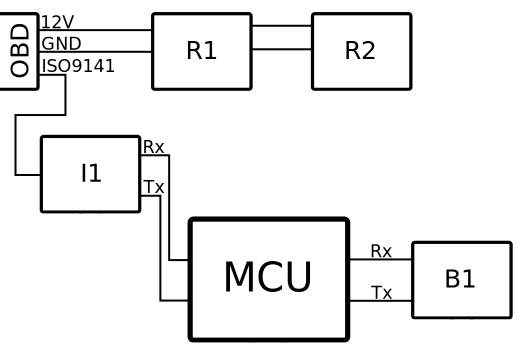
\includegraphics[scale=0.6]{Images/SchematBlokowyPlytki.pdf}
			\caption{Schemat blokowy zaprojektowanego interfejsu komunikacyjnego. Opis w tekście.}
			\label{rys_schemat_blokowy_plytki}
		\end{figure}	
	
	Na schemacie zaprezentowano następujące elementy: 
	
	\begin{itemize}
		\item{OBD - komputer pokładowy pojazdu,}
		\item{R1 - regulator napięcia 5V - źródło zasilania dla interfejsu komunikacyjnego I1,}
		\item{R2 - regulator napięcia 3.3V - źródło zasilania dla mikroprocesora MCU oraz modułu bluetooth B1,}
		\item{I1 - interfejs komunikacyjny ISO9141,}
		\item{MCU - mikroprocesor,}
		\item{B1 - moduł komunikacyjny bluetooth.}
	\end{itemize}
	
	W założeniach interfejs miał umożliwić bezprzewodową komunikację pomiędzy komputerem Raspberry Pi, a złączem diagnostycznym. W kolejnych podrozdziałach znajduje się dokładny opis projektu.	
	
	\newpage
	\subsection{Schemat elektryczny}
	
		\hspace{0.5cm}Celem zaprojektowanego układu było umożliwienie komunikacji z samochodowym komputerem pokładowym poprzez złącze diagnostyczne. Głównym elementem układu jest mikroprocesor U1, którego zadaniem jest odbieranie danych ze złącza diagnostycznego oraz przesyłanie odebranych danych za pomocą modułu bluetooth do układu wizualizacji danych. Mikroprocesor zasilany jest napięciem 3.3V. Układ został zaprojektowany do obsługi tylko jednego protokołu komunikacyjnego udostępnianego przez złącze diagnostyczne - ISO 9141-2. Wynika to z potrzeby minimalizacji całego układu, a także minimalizacji ceny jego wykonania. Sygnał protokołu komunikacyjnego doprowadzony jest do złącza P1 wraz z napięciem 12V - którego źródłem jest akumulator - oraz wyprowadzeniami masy układu. Sygnał zasilania złącza P1 doprowadzony jest to dwóch regulatorów napięcia U4 oraz U5, dzięki którym w układzie dostępne są napięcia zasilające odpowiednio 5V oraz 3.3V. W obwodzie wejściowym oraz wyjściowym umieszczone zostały kondensatory C1, C2 i C3 zgodnie z zaleceniami producenta \cite{MC7805}\cite{MCP17}. W obwodzie zasilania znajduje się dioda prostownicza D8 oraz dodatkowo dwie czerwone diody LED D4 i D5 wraz z odpowiadającymi im rezystorami R4 i R5, których zadaniem jest sygnalizowanie obecności napięcia.
		
		Sygnał linii k protokołu ISO 9141-2 wychodzący ze złącza P1 doprowadzony jest do układu interfejsu magistrali ISO 9141. Układ ten zasilany jest napięciem 5V, a jego zadaniem jest przetwarzanie sygnału wyprowadzonego ze złącza diagnostycznego. Zastosowanie takiego rozwiązania umożliwia wygodne programowanie komunikacji ze złączem diagnostycznym przy użyciu interfejsu UART, które  jest bezpośrednio dostępne w zastosowanym mikroprocesorze. Ze względu na różnicę napięć pracy układu L9637D oraz mikroprocesora do odbierania danych z wyprowadzenia Rx interfejsu ISO należy dodatkowo obniżyć napięcie sygnału. Do tego celu wykorzystano rezystancyjny dzielnik napięcia R8 i R9. Wysyłanie danych z mikroprocesora może odbywać się bezpośrednio, ponieważ napięcie 3.3V jest wystarczające do zmiany stanu na wejściu Tx układu U3. W obwodzie komunikacji pomiędzy modułami umieszczono dodatkowo złącze umożliwiające bezpośrednie odczytywanie danych na liniach Rx oraz Tx, które może być wykorzystywane w celach diagnostycznych lub jako wyprowadzenie do dodatkowego mikroprocesora. Dokładny opis układu można znaleźć w nocie katalogowej producenta \cite{L9637D}.
		
		Układ U2 znajdujący się na schemacie to moduł komunikacyjny bluetooth. Jego zadaniem jest odbieranie wstępnie opracowanych wyników ze złącza diagnostycznego do układu wizualizacji danych. Moduł charakteryzuje się małym poborem prądu w stanie pracy(12mA), bardzo małym w stanie spoczynku(<0.5A), a także dużą szybkością przesyłania danych(do 1Mbps). Dokładną specyfikację urządzenia można znaleźć w nocie katalogowej producenta \cite{RN4020}. Układ zasilany jest napięciem 3.3V oraz komunikuje się z mikroprocesorem wykorzystując magistralę UART. Dodatkowo do modułu U2 doprowadzony jest sygnał wybudzający ze stanu czuwania(7:WAKE\_ SW) oraz sygnał wejścia resetującego układ(8:CMD/MLDP). Wyprowadzenia PIO1, PIO2, PIO3 wykorzystane zostały do sygnalizowania stanu komunikacji układu. Dodatkowo moduł bluetooth posiada wyprowadzenia magistrali SPI, które w zaprojektowanym układzie nie zostały wykorzystane. 
		
		\newpage		
		
		W układzie znajdują się również elementu obsługi mikroprocesora. Złącze P3 umożliwia programowanie mikroprocesora z wykorzystaniem zewnętrznego programatora dostępnego w zestawach STM32 NUCLEO lub DISCOVERY lub programatora ST-LINK/V2. Dodatkowo w układzie znajdują się dwa rezonatory kwarcowe(Q1, Q2) wraz kondensatorami(C7, C8, C9, C10) zgodne z zaleceniami producenta, a także przycisk umożliwiający resetowanie układu(S1). 
		
		Rys. \ref{rys_schemat_ukladu_elektrycznego} przedstawia schemat zaprojektowanego układu. Schemat w większym rozmiarze dodany został również do załączników na końcu dokumentu.
		
		\begin{figure}[!h]
			\centering
			\includegraphics[scale=0.6, angle=90]{Images/SchematUkladuElektrycznego.pdf}
			\caption{Schemat obwodu układu do komunikacji ze złączem diagnostycznym. Opis w tekście.}
			\label{rys_schemat_ukladu_elektrycznego}
		\end{figure}
	
		\newpage
	
	
	\subsection{Zastosowane elementy}W projekcie układu do komunikacji ze złączem diagnostycznym wykorzystane zostały układy scalone wymienione poniżej(w nawiasie znajduje się symbol odpowiadający danemu elementowi na Rys. \ref{rys_schemat_ukladu_elektrycznego}.
	
	\begin{itemize}
		\item{Mikroprocesor F103CBT6 firmy STM32(U1). W tabeli \ref{tab_stm32} przedstawione zostały jego najważniejsze w kontekście omawianego układu dane katalogowe.
			\begin{table}[!h]
			\centering
			\caption{Najważniejsze parametry STM32F103CBT6 \cite{stm32}.}
			\label{tab_stm32}
			\begin{tabular}{|c|c|c|c|}
			\hline
			\textbf{\begin{tabular}[c]{@{}c@{}}Napięcie\\ zasilania\end{tabular}} & \textbf{\begin{tabular}[c]{@{}c@{}}Częstotliwość\\ Taktowania\end{tabular}} & \textbf{\begin{tabular}[c]{@{}c@{}}Pamięć\\ Flash\end{tabular}} & \textbf{\begin{tabular}[c]{@{}c@{}}Pamięć\\ SRAM\end{tabular}} \\ \hline
3.3V & 72MHz & 128kB  & 20kB \\ \hline \hline 
\textbf{\begin{tabular}[c]{@{}c@{}}Liczba\\ timerów\end{tabular}} & \textbf{Interfejsy} & \textbf{Obudowa} & \textbf{Montaż}\\ \hline 
4, 16bit & \begin{tabular}[c]{@{}c@{}}CAN, I2C x2, LIN\\ SPI x2, USART x2\end{tabular} & LQFP48 & SMD \\ \hline
	\end{tabular}
	\end{table}
		}
		
		\item{Moduł komunikacji bluetooth RN4020-V/RM firmy Microchip(U2). W tabeli \ref{tab_RN4020} przedstawione zostały jego najważniejsze dane katalogowe.
		
		\begin{table}[!h]
		\centering
		\caption{Najważniejsze parametry RN4020-V/RM \cite{RN4020}.}
		\label{tab_RN4020}
		\begin{tabular}{|c|c|c|c|}
		\hline
\textbf{\begin{tabular}[c]{@{}c@{}}Napięcie\\ zasilania\end{tabular}} & \textbf{Standard}                                                      & \textbf{Komunikacja}                                                & \textbf{Protokół}                                           \\ \hline
3.0-3.6V                                                              & 4.1                                                                    & UART                                                                & \begin{tabular}[c]{@{}c@{}}ASCII AT\\ Commands\end{tabular} \\ \hline \hline
\textbf{\begin{tabular}[c]{@{}c@{}}Programowalne\\ GPIO\end{tabular}} & \textbf{\begin{tabular}[c]{@{}c@{}}Częstotliwość\\ pracy\end{tabular}} & \textbf{\begin{tabular}[c]{@{}c@{}}Wbudowana\\ antena\end{tabular}} & \textbf{Montaż}                                             \\ \hline
\begin{tabular}[c]{@{}c@{}}7 cyfrowych\\ 3 analogowe\end{tabular}                                                                  & 2.402-2.480GHz                                                         & Tak                                                                 & SMD                                                         \\ \hline
\end{tabular}
\end{table}
		
		}		
	
	\item{Interfejs protokołu ISO9141-2, L9637D firmy STMicroelectronics(U3). Dane katalogowe tego układu znaleźć można w odnośniku \cite{L9637D}.}
	\item{Regulator napięcia 5V MC7805BDTRK(U4). Dane katalogowe tego układu znaleźć można w odnośniku \cite{MC7805}.}
	
	\item{Regulator napięcia 3.3V MCP1703T-3302E/CB(U5). Dane katalogowe tego układu znaleźć można w odnośniku \cite{MCP17}.}
	
	\end{itemize}	
	
	\newpage
	
	W tabeli \ref{tab_wykaz_czesci} znajduje się pełny wykaz wykorzystanych elementów.
	
	\begin{table}[!h]
\centering
\caption{Wykaz wykorzystanych elementów wraz z opisem obudowy, rodzaju montażu oraz warstwy na projekcie obwodu drukowanego.}
\label{tab_wykaz_czesci}
\begin{tabular}{|c|c|c|c|c|c|}
\hline
\textbf{Oznaczenie} & \textbf{Nazwa/wartość} & \textbf{Obudowa} & \textbf{Montaż} & \textbf{Ilość} & \textbf{Warstwa} \\ \hline
U1                  & STM32F103CBT6          & LQFP48           & SMD             & 1              & Górna            \\ \hline
U2                  & RN4020-V/RM            & RN4020-ALT       & SMD             & 1              & Dolna            \\ \hline
U3                  & L9637D                 & SO8              & SMD             & 1              & Górna            \\ \hline
U4                  & \begin{tabular}[c]{@{}c@{}}MC78M05\\ BDTRK\end{tabular}           & TO-252-3  & SMD             & 1              & Górna            \\ \hline
U5                  & \begin{tabular}[c]{@{}c@{}}MCP1703T-3302\\ E/CB\end{tabular}      & SOT-23-3         & SMD             & 1              & Górna            \\ \hline
R1, R2, R3          & 330$\Omega$                   & 0402             & SMD             & 3              & Dolna            \\ \hline
R4, R5              & 330$\Omega$                   & 0402             & SMD             & 2              & Górna            \\ \hline
R7                  & 510$\Omega$                   & 0402             & SMD             & 1              & Górna            \\ \hline
R8                  & 12k$\Omega$                   & 0402             & SMD             & 1              & Górna            \\ \hline
R9                  & 22k$\Omega$                   & 0402             & SMD             & 1              & Górna            \\ \hline
R10                 & 1M$\Omega$                    & 0402             & SMD             & 1              & Dolna            \\ \hline
R11                 & 10k$\Omega$                   & 0402             & SMD             & 1              & Dolna            \\ \hline
C1, C2, C12         & 1$\mu$F 16V                & 0402             & SMD             & 3              & Górna            \\ \hline
C3                  & 1$\mu$F 25V                & 0603             & SMD             & 1              & Górna            \\ \hline
C5                  & 100nF 16V              & 0402             & SMD             & 1              & Dolna            \\ \hline
C6                  & 100nF 16V              & 0402             & SMD             & 1              & Górna            \\ \hline
C7, C8              & 22pF 50V               & 0402             & SMD             & 2              & Dolna            \\ \hline
C9, C10             & 10pF 50V               & 0402             & SMD             & 2              & Dolna            \\ \hline
C11                 & 4.7$\mu$F 10V              & 0402             & SMD             & 1              & Dolna            \\ \hline
D1, D2, D3          & Red diode              & 0402             & SMD             & 3              & Dolna            \\ \hline
D4, D5              & Red diode              & 0402             & SMD             & 2              & Górna            \\ \hline
D8                  & 1N4007                 & DO-41            & THT             & 1              & Górna            \\ \hline
Q1                  & 32.768kHz              & 3.2x1.5x0.9    & SMD             & 1              & Dolna            \\ \hline
Q2                  & 8MHz                   & HC49U            & THT             & 1              & Dolna            \\ \hline
P1                  & Header                 & HDR1X4           & THT             & 1              & Górna            \\ \hline
P3                  & Header                 & HDR1X5           & SMD             & 1              & Górna            \\ \hline
P4                  & Header                 & HDR1X3           & THT             & 1              & Górna            \\ \hline
S1                  & Button PS-03B          & SPST-NO          & THT             & 1              & Górna            \\ \hline
CB1                 & Button PS11ABK         & SPST-NO          & THT             & 1              & Górna            \\ \hline
\end{tabular}
\end{table}

\newpage


	\subsection{Projekt obwodu drukowanego}
		\hspace{0.5cm}Na podstawie zaprojektowanego schematu elektrycznego zaprojektowany został obwód drukowany. Przy projektowaniu istotnym aspektem był rozmiar oraz kształt wykonanej płytki, aby układ mógł zostać umieszczony w obudowie, której widok oraz przekrój poprzeczny wraz z wymiarami przedstawiony został na Rys. \ref{widok_wtyczka_obd}.
		
		\begin{figure}[!h]
			\centering
			\subfigure[]{
				\includegraphics[scale=0.3]{Images/widok_wtyczka_obd.png}
			} 
			\subfigure[]{
				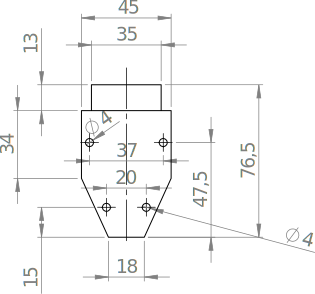
\includegraphics[scale=1]{Images/wymiary_wtyczka_obd.pdf}
			} 
			\caption{Widok (a) oraz przekrój poprzeczny z wymiarami (b) obudowy układu do komunikacji ze złączem diagnostycznym.}
			\label{widok_wtyczka_obd}
		\end{figure} 
	
	Projekt obwodu drukowanego został wykonany w technologii dwustronnej. W tabeli \ref{tab_opis_warstw_pcb} znajduje się opis poszczególnych warstw zaprojektowanej płytki.
	
	\begin{table}[!h]
\centering
\caption{Opis wykorzystanych warstw.}
\label{tab_opis_warstw_pcb}
\begin{tabular}{|c|c|c|c|}
\hline
\textbf{Nazwa/Typ}                                                & \textbf{Materiał}                                         & \textbf{Grubość {[}mm{]}} & \textbf{\begin{tabular}[c]{@{}c@{}}Stała\\ dielektryczna\end{tabular}} \\ \hline
Pokrycie górne                                                    &                                                           &                           &                                                                        \\ \hline
Górna soldermaska                                                 & Poliamid                                                  & 0.01016                   & 3.5                                                                    \\ \hline
\begin{tabular}[c]{@{}c@{}}Górna warstwa\\ sygnałowa\end{tabular} & Miedź                                                     & 0.03556                   &                                                                        \\ \hline
\begin{tabular}[c]{@{}c@{}}Warstwa\\ dielektryczna\end{tabular}   & \begin{tabular}[c]{@{}c@{}}Dielektryk\\ FR-4\end{tabular} & 0.32004                   & 4.8                                                                    \\ \hline
\begin{tabular}[c]{@{}c@{}}Dolna warstwa\\ Sygnałowa\end{tabular} & Miedź                                                     & 0.03556                   &                                                                        \\ \hline
Dolna soldermaska                                                 & Poliamid                                                  & 0.01016                   & 3.5                                                                    \\ \hline
Pokrycie dolne                                                    &                                                           &                           &                                                                        \\ \hline
\end{tabular}
\end{table}

		\newpage
	
		W tabeli \ref{tab_wykaz_czesci}	znajduje się wykaz zastosowanych elementów wraz z warstwą, na której zostały umieszczone. Na Rys. \ref{warstwa_top} \ref{warstwa_bottom} przedstawione zostały schematy obwodów obu warstw, a także widoki modelu. 
	
		\begin{figure}[!h]
			\centering
			\subfigure[]{
				\includegraphics[scale=0.4]{Images/rys_pcb_top_schemat.png}
			} 
			\subfigure[]{
				\includegraphics[scale=0.4]{Images/rys_pcb_top_model.png}
			} 
			\caption{Schemat obwodu (a) oraz widok modelu (b) górnej warstwy płytki.}
			\label{warstwa_top}
		\end{figure} 		
		
		\begin{figure}[!h]
			\centering
			\subfigure[]{
				\includegraphics[scale=0.4]{Images/rys_pcb_bottom_schemat.png}
			} 
			\subfigure[]{
				\includegraphics[scale=0.4]{Images/rys_pcb_bottom_model.png}
			} 
			\caption{Schemat obwodu (a) oraz widok modelu (b) dolnej warstwy płytki.}
			\label{warstwa_bottom}
		\end{figure} 
		
		\newpage
		
		
	
		\newpage

%---------------------------------------------------OPROGRAMOWANIE-------------------------------------------------------------	

\section{Zbudowany układ i oprogramowanie}

\hspace{0.5cm}Jako jednostkę centralną w układzie zastosowano komputer Raspberry Pi 3, na którym zainstalowano system Raspbian Jessie. Główną zaletą tego urządzenia jest wbudowany moduł bluetooth, dzięki czemu zbędne stają się dodatkowe urządzenia do komunikacji z interfejsem ELM 327.  W tabeli \ref{tab_raspberry_pi} pokazano najważniejsze parametry komputera, a na Rys. \ref{rys_raspberry_pi} przedstawiono jego widok.

\begin{table}[!h]
\centering
\caption{Wybrane parametry komputera Raspberry Pi 3 \cite{raspberrypiwidok}.}
\label{tab_raspberry_pi}
\begin{tabular}{|c|c|c|c|}
\hline
\textbf{Procesor}                                                  & \textbf{Bluetooth}                                       & \textbf{Wifi} & \textbf{Display} \\ \hline 
\begin{tabular}[c]{@{}c@{}}4 x 1.2GHz \\ 64-bit ARMv8\end{tabular} & 4.1 BLE                                                  & 802.11n       & Full HDMI        \\ \hline \hline
\textbf{GPIO}                                                      & \textbf{Interfejsy}                                      & \textbf{RAM}  & \textbf{Dysk}    \\ \hline
40                                                                 & \begin{tabular}[c]{@{}c@{}}I2C, UART,\\ SPI\end{tabular} & 1 GB          & Micro SD         \\ \hline
\end{tabular}
\end{table}	
	
		\begin{figure}[!h]
			\centering
			\includegraphics[scale=0.6]{Images/rys_raspberry_pi.png}
			\caption{Widok komputera Raspberry Pi 3 \cite{raspberrypiwidok}.}
			\label{rys_raspberry_pi}
		\end{figure}	

\newpage

	Do wyświetlania interfejsu komunikacyjnego wykorzystano siedmiocalowy, dotykowy wyświetlacz ciekłokrystaliczny firmy waveshare, którego wybrane parabetry przedstawiono w tabeli \ref{tab_wyswietlacz}, natomiast na Rys. \ref{rys_wyswietlacz} pokazano jego widok.

	\begin{table}[!h]
\centering
\caption{Wybrane parametry wyświetlacza waveshare \cite{wyswietlaczwidok}.}
\label{tab_wyswietlacz}
\begin{tabular}{|c|c|c|c|}
\hline
\textbf{Przekątna} & \textbf{Rozdzielczość} & \textbf{\begin{tabular}[c]{@{}c@{}}Typ\\ wyświetlacza\end{tabular}}    & \textbf{Złącze} \\ \hline
7''                & 1024x600px             & \begin{tabular}[c]{@{}c@{}}IPS, dotykowy,\\ pojemnościowy\end{tabular} & HDMI            \\ \hline
\end{tabular}
\end{table}

		\begin{figure}[!h]
			\centering
			\includegraphics[scale=0.25]{Images/rys_wyswietlacz.png}
			\caption{Widok komputera Raspberry Pi 3 \cite{wyswietlaczwidok}.}
			\label{rys_wyswietlacz}
		\end{figure}
		W celu umożliwienia poprawnej współpracy wyświetlacza z komputerem Raspberry niezbędna była zmiana konfiguracji systemu, zgodnie z zaleceniami producenta \cite{wyswietlaczconf}.
		
		Ostatnim elementem zbudowanego układu jest interfejs komunikacyjny ELM 327, którego dokładny opis znajduje się w rozdziale \ref{rozdzial_elm}.

\newpage

\hspace{0.5cm}W ramach pracy stworzono oprogramowanie umożliwiające komunikację ze złączem diagnostycznym poprzez urządzenie ELM327, zapisywanie danych pomiarowych oraz wizualizację odczytywanych parametrów. Zgodnie z przyjętymi standardami dobrego wytwarzania oprogramowania, aplikacja podzielona została na dwa osobne moduły. Moduł pierwszy odpowiedzialny jest za zarządzanie logiką aplikacji, drugi natomiast za komunikację z użytkownikiem za pomocą graficznego interfejsu. Na Rys. \ref{rys_ogolny_schemat_aplikacji} przedstawiony został schemat ideowy aplikacji.

		\begin{figure}[!h]
			\centering
			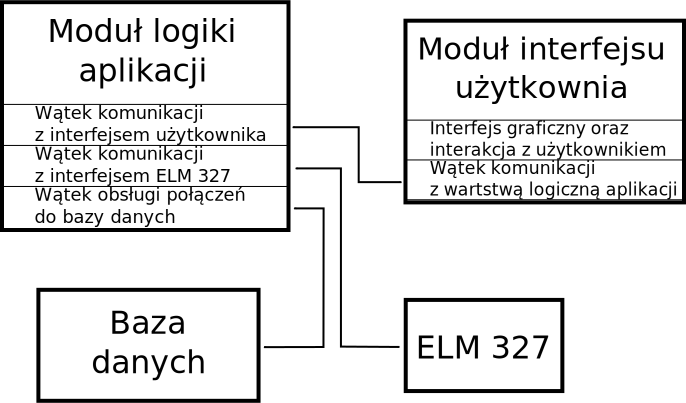
\includegraphics[scale=0.75]{Images/rys_ogolny_schemat_aplikacji.pdf}
			\caption{Schemat ideowy aplikacji.}
			\label{rys_ogolny_schemat_aplikacji}
		\end{figure}

W kolejnych dwóch podrozdziałach znajduje się dokładny opis zastosowanych rozwiązań.

\newpage

%---------------------------------------------------APLIKACJA KOMUNIKACYJNA-------------------------------------------------------------	
	
\subsection{Moduł komunikacji i przetwarzania danych}\label{rozdzial_raspberry_software}
	\subsubsection{Struktura aplikacji}\label{rozdzial_pakiety_api}
	\hspace{0.5cm}Zadaniem omawianego w tym rozdziale modułu jest dostarczenie aplikacji usług niezbędnych do komunikowania się z interfejsem ELM 327 oraz przechowywania odczytywanych wyników pomiarów. Aplikacja napisana została w języku Java 8 kompilowana z wykorzystaniem narzędzia Maven z wykorzystaniem dodatkowych bibliotek:

	\begin{itemize}
		\item{do obsługi portu szeregowego: jbidibc-rxtx-2.2 1.6.0 implementująca bibliotekę rxtx 2.1.7,}
		\item{do obsługi loggera aplikacji: log4j 1.2.17}
		\item{do obsługi połączenia z bazą danych: hibernate-core 5.2.6 oraz mysql-connector-java 5.1.38.}
	\end{itemize}
	
	Moduł został podzielony na pakiety zgodnie z przedstawionym na Rys. \ref{rys_pakiety_api}.
	
		\begin{figure}[!h]
			\centering
			\includegraphics[scale=1]{Images/rys_pakiety_api.png}
			\caption{Schemat ideowy aplikacji.}
			\label{rys_pakiety_api}
		\end{figure}
		
	W folderze Source Packages znajdują się wszystkie pakiety aplikacji:
	
	\begin{itemize}
		\item{pl.mbartosz.api.ElmService - zawiera wszystkie klasy obsługujące komunikację z interfejsem ELM 327,}
		\item{pl.mbartosz.api.dao - zawiera klasy interfejsów operujących na bazie danych,}
		\item{pl.mbartosz.api.domain - zawiera klasy encji bazy danych. Klasy te generują automatycznie tabele w bazie danych jeżeli jeszcze nie istnieją,}
		\item{pl.mbartosz.api.raspberry.serialservices - zawiera klasy obsługujące konfigurację, połączenie i komunikację z wykorzystaniem portu szeregowego,}
		\item{pl.mbartosz.api.services - zawiera interfejsy pośredniczące w wymianie danych pomiędzy klasami operującymi bezpośrednio na bazie danych, a klasami aplikacji, }
		\item{pl.mbartosz.api.services.impl - zawiera klasy implementujące interfejsy z pakieto *.services,}
		\item{pl.mbartosz.api.services.util - zawiera klasę konfiguracyjną połączenia z bazą danych.}
	\end{itemize}
	
	Folder Test Packages zawiera klasy automatycznych testów. Do aplikacji nie zostały napisane żadne testy, dlatego folder ten jest pusty. Kolejny folder - Other Sources - zawiera plik konfiguracyjny biblioteki hibernate umożliwiający połączenie aplikacji z bazą danych. W folderze Project Files znajdują się pliki konfiguracyjne dla narzędzia Maven, oraz środowiska NetBeans.
	
	\subsubsection{Funkcjonalność aplikacji}	
	
	\hspace{0.5cm}Aplikacja udostępnia trzy funkcjonalności: komunikację z portem szeregowym, komunikacje z ELM 327 wykorzystująca port szeregowy oraz obsługę zapisywania i pozyskiwania danych z bazy. Obsługa komunikacji z portem szeregowym zawarta w pakiecie pl.mbartosz.api.raspberry.serialservices umożliwia połączenie z portem wykorzystując wykorzystując zdefiniowane przez użytkownika parametry, a także wysyłanie danych do portu oraz odbieranie informacji zwrotnych w trybie zapytania i oczekiwania na odpowiedź. W pakiecie znajdują się trzy klasy:
	
	\begin{itemize}
		\item{SerialPortComm - zawiera funkcje umożliwiające wyszukiwanie dostępnych w systemie portów, podłączenie oraz rozłączenie od portu szeregowego,}
		\item{SerialPortCongurationParameters - zawiera obiekty konfiguracyjne dla połączenia z portem,}
		\item{AtCommandPort - zawiera funkcje umożliwiające komunikację z wykorzystaniem portu szeregowego.}
	\end{itemize}
	
	Najistotniejsze z punktu widzenia funkcjonalności aplikacji są metody odpowiedzialne za wysyłanie instrukcji do portu szeregowego oraz odbieranie informacji zwrotnych. Funkcja wysyłająca dane do portu zaprezentowana została na Listingu \ref{listing_put_command}. Przyjmuje ona jeden argument w postaci łańcucha znaków. Podawana jest tutaj instrukcja, która ma zostać wysłana do portu. Zmienna responseData służy do przechowywania otrzymanej odpowiedzi w postaci listy tablic typu byte. Na początku następuje wyzerowanie zmiennej przechowującej liczbę otrzymanych odpowiedzi, a następnie do portu wysyłana jest żądana komenda po konwersji to tablicy typu byte. W kolejnym kroku wykonywana jest pętla, powtarzająca się dopóki nie liczba otrzymanych odpowiedzi nie jest równa liczbie oczekiwanych odpowiedzi. Takie rozwiązanie umożliwia wysłanie jednej komendy i otrzymanie kilku linii odpowiedzi co jest wykorzystywane przy wysyłaniu niektórych instrukcji do OBD-II. Po wysłaniu instrukcji wątek przechodzi w stan oczekiwania na odpowiedź.
	
	\newpage
	
	\lstinputlisting[language=JavaL, caption={Funkcja wysyłająca dane do portu szeregowego. Opis w tekście.}, label={listing_put_command}]{Listings/put_command.java}
	
	Funkcja odpowiadająca za odbieranie danych z portu szeregowego implementuje interfejs SerialPortEventListener, dzięki czemu możliwa jest wykonanie określonych instrukcji dokładnie w momencie pojawienia się danych na porcie. Wysyłanie danych oraz ich odbieranie synchronizowane jest poprzez obiekt responseSync. W każdym wywołaniu wydarzenia na porcie odbierana jest tylko jedna linia danych i zapisywana do listy tablic typu byte. Następnie zwalniana jest blokada obiektu responseSync i program wraca do linii siódmej funkcji wysyłającej dane do portu. Obsługa odbierania danych przestawiona została na Listingu \ref{listing_serial_listener}. \\
	
	\lstinputlisting[language=JavaL, caption={Funkcja odbierająca dane z portu szeregowego.  Opis w tekście.}, label={listing_serial_listener}]{Listings/serial_listener.java}
	
	\newpage
	
	Realizacja komunikacji z interfejsem ELM 327 zawarta jest w pakiecie pl.mbartosz.api.ElmService, który zawiera następujące klasy:
	
	\begin{itemize}
		\item{AT\_ COMMANDS - jest to klasa wyliczeniowa, w której zdefiniowane są komendy AT, ich opis, a także oczekiwana odpowiedź dla każdej komendy,}
		\item{CommandObject - obiekt przechowujący komendę, oraz oczekiwaną liczbę linii odpowiedzi,}
		\item{ResponseObject - obiekt przechowujący listę odpowiedzi oraz ich status,}
		\item{CommunicationMode - klasa wyliczeniowa, w której zdefiniowane są tryby pracy z urządzeniem : AUTO, MANUAL i WAIT,}
		\item{CommunicationState - klasa wyliczeniowa, w której zdefiniowany jest stan połączenia z urządzeniem: CONNECTED, DISSCONNCTED,}
		\item{ElmMessageService - klasa udostępniająca metody do wysyłania i odbierania danych z urządzenia.}
	\end{itemize}
	
	Większość klas w tym pakiecie to obiekty przechowujące parametry pracy aplikacji. Najważniejsza z punktu widzenia funkcjonalności jest klasa ElmMessageService, która zarządza wątkiem wysyłającym instrukcje do interfejsu ELM 327, generuje instrukcje do wysłania, a także przetwarza odebrane informacje. W celu optymalizacji pracy aplikacji komunikacja przeniesiona jest do osobnego wątku, który widocznym jest na Listingu \ref{listing_communication_thread}. \\
	
	\lstinputlisting[language=JavaL, caption={Wątek komunikacji z ELM 327.  Opis w tekście.}, label={listing_communication_thread}]{Listings/communication_thread.java}
	
	
	\newpage
	
	Metoda run() jest implementacją interfejsu Runnable pozwalającego na uruchamianie nowych wątków. Po uruchomieniu wątku wykonywana jest instrukcja nieskończonej pętli, której działanie może zakończyć tylko wyłączenie programu. W pętli tej sprawdzane są warunki stanu aplikacji. Jeżeli aplikacja jest w trybie pracy automatycznej to znaczy w przypadku wyświetlania panelu głównego lub zaznaczenia odpowiedniej opcji w ustawieniach aplikacji(rozdział \ref{rozdzial_hmi_software}) do urządzenia wysyłana jest instrukcja w trybie ciągłym, synchronizowanym obiektem responseSync. W przypadku gdy aplikacja pracuje w trybie ręcznym lista instrukcji zostaje wysłana do urządzenia tylko raz. Następnie aplikacja zmienia stan pracy na oczekiwanie. W trybie oczekiwania wątek jest wstrzymywany na 10ms, po czym następuje ponowne sprawdzenie warunków wykonywania instrukcji \mbox{wątku}. 
	
	Za generowanie oraz wysyłanie instrukcji do urządzenia odpowiada funkcja sendToPort, której struktura przedstawiona na Listingu \ref{listing_send_to_port}. W metodzie tej najważniejszą funkcję pełni pętla for. Ponieważ pojedyncze zapytanie do urządzenia może zawierać kilka instrukcji, pętla ma za zadanie pobierać z listy instrukcji po kolei każdą z nich i wysyłania jej metodą putAtCommand. Funkcja ta zwraca obiekt typu ResponseObject, który następnie dodawany jest do listy otrzymanych odpowiedzi. Kiedy wykonane zostają wszystkie instrukcje z zapytania i otrzymano odpowiedzi od urządzenia wywoływana jest metoda sprawdzająca poprawność odebranych informacji executeResponse. 
	\\
	
	\lstinputlisting[language=JavaL, caption={Funkcja generująca instrukcje do wysłania. Opis w tekście.}, label={listing_send_to_port}]{Listings/send_to_port.java}
	
	\newpage
	
	Zadaniem metody executeResponse jest sprawdzenie poprawności otrzymanych odpowiedzi dla każdej instrukcji oraz wymuszenie odświeżenia komponentów interfejsu użytkownika. Metoda ta w pętli sprawdza w pierwszej kolejności czy flaga poprawności w każdym odebranym obiekcie 	jest zaznaczona. Następnie w kolejnej pętli porównuje wszystkie odebrane odpowiedzi dla jednego obiektu responseObject z oczekiwanymi odpowiedziami. Odpowiedzialna jest za to funkcja checkResponse, która jako argument przyjmuje dwa łańcuchy znaków. Pierwszy argument to otrzymana odpowiedź, drugi natomiast to odpowiedź oczekiwana w postaci wyrażenia regularnego zdefiniowanego dla każde instrukcji w klasie AT\_ COMMANDS. Po sprawdzeniu poprawności odpowiedzi następuje wymuszenie odświeżenia interfejsu użytkownika. Omawiane funkcje przedstawione są na Listinigu \ref{listing_execute_response}.
	\\
	
	\lstinputlisting[language=JavaL, caption={Funkcja sprawdzająca poprawność odpowiedzi i wymuszająca odświeżenie interfejsu użytkownika. Opis w tekście.}, label={listing_execute_response}]{Listings/execute_response.java}	
	
	Pozostałe pakiety wymienione w podrozdziale \ref{rozdzial_pakiety_api} odpowiadają za komunikację aplikacji z bazą danych i są w istocie implementacją framworku Hibernate, dlatego ich dokładny opis został w pracy pominięty.
	
	\newpage
	
	\subsubsection{Baza danych}
	
	\hspace{0.5cm}Aplikacja połączona jest z relacyjną bazą danych MySQL umożliwiającą zapisywanie odczytywanych wyników w celu ich dalszej analizy. Na Rys. \ref{rys_database_model} przedstawiony został model logiczny oraz fizyczny bazy danych.
	
		\begin{figure}[!h]
			\centering
			\subfigure[]{
				\includegraphics[scale=0.8]{Images/rys_logical_database_model.png}
			} 
			\subfigure[]{
				\includegraphics[scale=0.8]{Images/rys_physical_database_model.png}
			} 
			\caption{Model logiczny (a) oraz fizyczny (b) bazy danych. Opis w tekście.}
			\label{rys_database_model}
		\end{figure} 	
	
	Baza danych składa się z trzech tabel. Tabela vehicle zawiera podstawowe informację o pojeździe. Tabela state przechowuje informacje o odczytanych prędkościach i obrotach silnika pojazdu. Tabela trouble\_ codes odczytanych kodach błędów pojazdu. Tabela vehicle jest połączona relacją jeden do wielu z pozostałymi tabelami.
	
		
	
	\newpage
	
%---------------------------------------------------INTERFEJS GRAFICZNY-------------------------------------------------------------	
	
\subsection{Moduł interfejsu użytkownika}\label{rozdzial_hmi_software}
	\hspace{0.5cm}Moduł interfejsu użytkownika napisany został w języku Java z wykorzystaniem najnowszego framweworku do tworzenia interfejsów graficznych JavaFX 8. Wygląda oraz obsługa aplikacji zostały dostosowane ekranu o rozdzielczości 1024x600 pikseli. Po uruchomieniu użytkownikowi ukazuje się ekran przedstawiony na Rys. \ref{user_interface_dashboard}.
	
		\begin{figure}[!h]
			\centering
			\includegraphics[scale=0.44]{Images/user_interface_dashboard.png}
			\caption{Panel główny interfejsu użytkownika.}
			\label{user_interface_dashboard}
		\end{figure}
		
		Na zaprezentowanym widoku przedstawiony jest panel główny z zaznaczonymi poszczególnymi sekcjami:
		
		\begin{enumerate}
			\item{Nagłówek okna. Widoczne są tutaj data, lokalizacja oraz aktualny czas.}
			\item{Okno główne. Prezentuje treść odpowiednią do wybranej opcji z menu. Widok na Rys. \ref{user_interface_dashboard} prezentuje domyślne okno główne.}
			\item{Lewy panel przycisków menu. Znajdują się tutaj kolejno od góry:
				\begin{itemize}
					\item{Przycisk informacyjny. Po jego naciśnięciu w oknie głównym pokazany jest widok domyślny.}
					\item{Przycisk przeglądarki. W oknie pokazana jest przeglądarka. Nieobsłużony.}
					\item{Przycisk nawigacji. W oknie pokazana jest nawigacja. Nieobsłużony.}
					\item{Przycisk radia. W oknie pokazana jest panel sterowania radiem. Nieobsłużony.}
				\end{itemize}						
			}
			\item{Prawy panel przycisków menu. Znajdują się tutaj kolejno od góry:
				\begin{itemize}
					\item{Przycisk ustawień. Po jego naciśnięciu w oknie głównym jest panel ustawień.}
					\item{Przycisk multimediów. W oknie pokazana jest panel zarządzania multimediami. Nieobsłużony.}
					\item{Przycisk statystyk. W oknie pokazana jest panel prezentujący statystki zebranych danych. Nieobsłużony.}
					\item{Przycisk czujników. W oknie pokazana jest stan czujników parkowania. Nieobsłużony.}
				\end{itemize}						
			}
			\item{Panel statusu. Informuje o podłączeniu urządzenia ELM 327 oraz dostępie do sieci.}
		\end{enumerate}
		
		Przełączanie widoków okna polega na zmianie zawartości okna głównego. Panele przycisków nie zmieniają swojej zawartości. Widok przycisków zmienia się tylko w przypadku najechania na przycisk lub jego naciśnięcia. W panelu statusu kolorem niebieskim zaznaczone jest uzyskanie połączenia, natomiast białym brak połączenia. Wartości widoczne na widoku NaN oznaczają, że dane nie są odbierane od urządzenia ELM 327. Kiedy aplikacja pracuje w trybie automatycznym dane te są automatycznie odświeżane po odebraniu kolejnych wyników. 
		
		Po naciśnięciu przycisku ustawień okno główne zmienia zawartość i ukazuje się widok przedstawiony na Rys. \ref{user_interface_dashboard}
		
		\begin{figure}[!h]
			\centering
			\includegraphics[scale=0.55]{Images/user_interface_settings_parameters_tab.png}
			\caption{Panel główny interfejsu użytkownika.}
			\label{user_interface_dashboard}
		\end{figure}		
		
		W panelu ustawień dostępne są dwie zakładki. Pierwsza z nich umożliwia skonfigurowanie urządzenia ELM 327, a także prezentuje opis oraz identyfikator podłączonego urządzenia. W celu wysłania ustawień do interfejsu należy nacisnąć przycisk Apply. Naciśnięcie przycisku Cancel powoduje powrót wszystkich kontrolek do poprzedniego stanu natomiast naciśnięcie przycisku Default powoduje przywrócenie wszystkich domyślnych ustawień.
		
		\newpage
		
		Druga zakładka dostępna w panelu ustawień umożliwia podgląd odbieranych danych od urządzenia ELM, a także pracę w trybie ręcznego wysyłania żądań. Zakładka ta podzielona jest na dwie części. Strona lewa odpowiada za wybór portu szeregowego do którego aplikacja ma się podłączyć. Przyciski Connect i Dissconnect odpowiadają za ustanawianie połączenia lub jego zakończenie. Przycisk Refresh wywołuje funkcję wyszukującą wszystkie dostępne w systemie porty szeregowe. W drugim wierszu znajduje się pole tekstowe Cmd w które należy wpisać instrukcję do wysłania do interfejsu. Przycisk Send wywołuje metodę wysyłającą instrukcję poprzez ustawienie stanu aplikacji na ręczny. Poniżej znajduje się pole tekstowe wyświetlające odpowiedzi urządzenia ELM. Pole to można wyczyścić naciskając na przycisk Clear lub zapisać jego zawartość do pliku poprzez naciśnięcie przycisku Save. W panelu znajduje się dodatkowo kontrolka Auto, której zaznaczenie przełącza aplikację w tryb pracy automatycznej. W panelu po prawej można skonfigurować parametry połączenia szeregowego. Dostępne opcje to: szybkość transmisji, liczba bitów danych, parzystość, liczba bitów stopu oraz kontrola przepływu. Aby nowe ustawienia zostały wprowadzone należy zakończyć bieżące połączenie z portem i zainicjować je na nowo. Widok drugiej zakładki panelu ustawień widoczny jest na Rys. \ref{user_interface_dashboard}.
		
		\begin{figure}[!h]
			\centering
			\includegraphics[scale=0.55]{Images/user_interface_settings_elm_tab.png}
			\caption{Panel główny interfejsu użytkownika.}
			\label{user_interface_dashboard}
		\end{figure}
	
	
	\newpage
	
	\section{Wyniki testów układu}	
	
	\hspace{0.5cm}Stworzone oprogramowanie poddane zostało testom praktyczny w samochodzie Seat Cordoba II. Połączenie zostało skonfigurowane tak, aby w odpowiedzi nie odsyłane było echo żądania oraz znaki białe. Z odpowiedzi dodatkowo usunięty jest nagłówek, ale dopiero po sprawdzeniu czy spełnia ona warunek podany w wyrażeniu regularnym. Sprawdzone zostały oba tryby pracy: automatyczny i ręczny. W pierwszy kroku wykonany został test trybu ręcznego pracy aplikacji. Wyniki kilku przykładowych zapytań przedstawiono na Rys. \ref{rys_wyniki_testu_recznego}.
	
		\begin{figure}[!h]
			\centering
			\includegraphics[scale=0.55]{Images/rys_test_reczny.png}
			\caption{Wyniki testu ręcznego trybu pracy programu.}
			\label{rys_wyniki_testu_recznego}
		\end{figure}
		
		Pierwsza instrukcja wysłana to zapytanie o identyfikator urządzenia. Następnie wysłane zostały dwie instrukcje konfigurujące strukturę odpowiedzi. Instrukcja 0100 to pytanie o dostępne kody PID z zakresu 01-20. Na podstawie odpowiedzi wyznaczono dostępne kody dla testowanego samochodu.
		
\begin{table}[!h]
\centering
\caption{Kodu PID udostępnione w samochodzie testowym.}
\label{tabela_test_pids}
\begin{tabular}{|c|c|c|c|c|c|c|c|c|c|c|c|c|c|c|c|}
\hline
\multicolumn{4}{|c|}{9} & \multicolumn{4}{c|}{8} & \multicolumn{4}{c|}{3} & \multicolumn{4}{c|}{B} \\ \hline
1    & 0    & 0   & 1   & 1    & 0   & 0   & 0   & 0    & 0   & 1   & 1   & 1    & 0   & 1   & 1   \\ \hline
01   & 02   & 03  & 04  & 05   & 06  & 07  & 08  & 09   & 0A  & 0B  & 0C  & 0D   & 0E  & 0F  & 10  \\ \hline \hline
\multicolumn{4}{|c|}{8} & \multicolumn{4}{c|}{0} & \multicolumn{4}{c|}{1} & \multicolumn{4}{c|}{1} \\ \hline
1    & 0    & 0   & 0   & 0    & 0   & 0   & 0   & 0    & 0   & 0   & 1   & 0    & 0   & 0   & 1   \\ \hline
11   & 12   & 13  & 14  & 15   & 16  & 17  & 18  & 19   & 1A  & 1B  & 1C  & 1D   & 1E  & 1F  & 20  \\ \hline
\end{tabular}
\end{table}

	
	
	\newpage
	
	Kolejna instrukcja 0101 to instrukcja sprawdzająca stan diody kontrolnej silnika. Następnie wysłanych zostało kilka instrukcji o bieżące parametry pracy samochodu. Na podstawie przeprowadzonych testów można powiedzieć, że tryb pracy ręcznej zachowuje się poprawnie.	
	
	W kolejnym kroku wykonano test automatycznego trybu pracy aplikacji dla parametrów udostępnionych w testowym pojeździe. Mierzonymi parametrami były: obciążenie silnika podawane w (0 - 100\%), temperatura cieczy chłodzącej (-40 - 215${}^\circ C$), prędkość obrotowa silnika (0 - 16383 obr/min), prędkość silnika (0 - 255 km/h) oraz temperatura powietrza zasysanego (-40 - 215${}^\circ C$). Otrzymane rezultaty zaprezentowane zostały na Rys. \ref{rys_wyniki_testu_automatycznego}
	
	\begin{figure}[!h]
			\centering
			\includegraphics[scale=0.55]{Images/rys_test_auto.png}
			\caption{Wyniki testu automatycznego trybu pracy programu.}
			\label{rys_wyniki_testu_automatycznego}
		\end{figure}
	
	
	Na podstawie obserwacji pracy programu można powiedzieć, że automatyczny tryb pracy programu również zachowuje się poprawnie.
	
	\newpage
	
	\section{Dyskusja potencjalnych zastosowań}
	
	\hspace{0.5cm}Podstawowym zastosowanie układu omawianego w niniejszej pracy mogłoby być wczesne informowanie o wystąpieniu błędu w pojeździe. W tym celu należałoby cyklicznie odpytywać komputer pokładowy czy wystąpił jakieś błędy. Takie odpytywanie mogłoby się odbywać na przykład przy każdym uruchomieniu pojazdu. W tym celu należałoby dodatkowo doprowadzić do komputera sterującego programem sygnał zapłonu. Jeżeli w pojeździe zostałby wykryty błąd to na wyświetlaczu pojawiłby się stosowny napis z informacją o błędzie oraz jego źródle.
	
	Innym zastosowaniem mogłoby być obliczanie wartości średniego spalania czy zasięgu pojazdu. W tym celu można wykorzystać następujące komendy:
	
	\begin{itemize}
		\item{01 5E - zwraca wartość aktualnego przepływu paliwa w l/h,}
		\item{01 0D - zwraca wartość aktualnej prędkości pojazdu w km/h,}
		\item{01 2F - zwraca wartość ilości paliwa w zbiorniku jako wartość procentowa pojemności zbiornika.}
	\end{itemize}
	
	Pobierając wartość aktualnego przepływu paliwa dostatecznie często przez określony okres czasu można z dobrą dokładnością wyliczyć spalanie średnie korzystając z wzoru:
	
	\begin{equation}
		Q_{sr} = \frac{\sum{Q_{ch}}}{n} \bigg[\frac{l}{h}\bigg],
	\end{equation}		

gdzie: $Q_{sr}$ to średnia wartość przepływu paliwa w l/h, $Q_{ch}$ to wartość chwilowa wartość przepływu paliwa w l/h, n to liczba próbek. Następnie w analogiczny sposób można obliczyć średnią prędkość pojazdu. Korzystając z obliczonych wartości można wyznaczyć wartość średniego spalania na kilometr oraz na każde 100 kilometrów:
	
	\begin{equation}
		C_{sr} = \frac{Q_{sr}}{v_{śr}} \bigg[\frac{l}{km}\bigg],
	\end{equation}

gdzie: $C_{sr}$ to średnia spalanie w l/km, $c_{sr}$ obliczona średnia prędkość pojazdu. Wartość tę można w łatwy sposób przeliczyć na spalanie pojazdu w litrach na 100 kilometrów.

	Wykorzystując obliczoną wartość średniego spalania samochodu na 100 kilometrów można wyznaczyć zasięg samochodu. Pobierając wartość ilości paliwa w zbiorniku i znając pojemność maksymalną zbiornika można wykorzystać wzory:
	
	\begin{equation}
		d = \frac{\frac{V_{a}}{100} * V_{max}}{C_{sr}} [km],
	\end{equation}
	
	gdzie: d - obliczony zasięg pojazdu, $V_{a}$ - aktualna ilość paliwa w zbiorniku jako wartość procentowa pojemności zbiornika.
		
	\newpage
	
	\section{Podsumowanie}
	
	\hspace{0.5cm}Układ umożliwiający komunikację ze złączem diagnostycznym został wykonany prawie w całości zgodnie z założeniami pracy inżynierskiej. W skład stworzonego układu wchodzą następujące elementy:

	\begin{itemize}
		\item{komputer Raspberry Pi 3,}
		\item{dotykowy, siedmiocalowy wyświetlacz LCD,}
		\item{interfejs komunikacyjny ELM 327.}
	\end{itemize}	
	W celu zrealizowania założonych zadań wykonano:
	
	\begin{itemize}
		\item{projekt układu do komunikacji ze złączem diagnostycznym składający się z schematu elektrycznego i obwodu drukowanego,}
		\item{oprogramowanie umożliwiające komunikację ze złączem diagnostycznym, wyświetlanie danych oraz interakcję z użytkownikiem,}
		\item{testy stworzonego oprogramowania.}
	\end{itemize}
	
	Założeniem było wykonanie własnego modułu umożliwiającego komunikację ze złączem diagnostycznym, jednakże ze względów finansowych prace zakończono na etapie projektu. Projekt jest kompletnym rozwiązaniem, którego wykonanie zostało przesłane do wyceny. Oprogramowanie wgrane na komputer Raspberry Pi 3 połączony dotykowym wyświetlaczem testowane było w samochodzie Seat Cordoba II. Stworzony układ pozwala na ciągłe wysyłanie zdefiniowanych zapytań do złącza i obserwowanie zwracanych informacji na wyświetlaczu, lub ręczne wprowadzenie dowolnego żądania. Dodatkowo w pracy omówiono potencjalne zastosowania stworzonego układu pod kątem wspomagania kierowania pojazdem. 
	
	\newpage	
	
\begin{thebibliography}{99}

		\bibitem{Schmidgall08}
		Schmidgall R., Zimmermann W., \emph{Magistrale Danych w Pojazdach. Protokoły i Standardy}, Wydawnictwa Komunikacji i Łączności WKŁ, Warszawa, 2008.

		\bibitem{Merkisz02}
		Merkisz J., Mazurek St., \emph{Pokładowe systemy diagnostyczne pojazdów samochodowych}, Wydawnictwa Komunikacji i Łączności WKŁ, Warszawa, 2002.		
		
		\bibitem{Sitek11}
		Sitek K., Syta S., \emph{Pojazdy Samochodowe. Badania stanowiskowe i diagnostyka}, Wydawnictwa Komunikacji i Łączności WKŁ, Warszawa, 2011.
		
		\bibitem{White06}
		White C., Randall M., \emph{Kody usterek}, Wydawnictwa Komunikacji i Łączności WKŁ, Warszawa, 2006.
		
		\bibitem{Grzejszczyk10}
		Fryśkowski B., Grzejszczyk E., \emph{Systemy transmisji danych}, Wydawnictwa Komunikacji i Łączności WKŁ, Warszawa, 10.
		
		\bibitem{Upton15}
		Upton E., Halfacree G., \emph{Raspberry Pi. Przewodnik użytkownika. Wydanie III}, Wydawnictwo Helion, Gliwice, 2015.
		
		\bibitem{raspberrypi}
		https://www.raspberrypi.org/documentation/
		
		\bibitem{raspberrypiwidok}
		https://www.raspberrypi.org/products/raspberry-pi-3-model-b/
		
		\bibitem{wyswietlaczwidok}
		http://www.waveshare.com/img/devkit/LCD/7inch-HDMI-LCD-C/7inch-HDMI-LCD-C-3.jpg
		
		\bibitem{wyswietlaczconf}
		http://www.waveshare.com/wiki/7inch\_HDMI\_LCD\_\%28C\%29	
	
		\bibitem{Schildt15}
		Schildt H., \emph{Java. Kompendium programisty. Wydanie IX}, Wydawnictwo Helion, Gliwice, 2015.
		
		\bibitem{saej1962}
		https://law.resource.org/pub/us/cfr/ibr/005/sae.j1962.2002.pdf (14.02.2017)
		
		\bibitem{saej1979}
		https://law.resource.org/pub/us/cfr/ibr/005/sae.j1979.2002.pdf (14.02.2017)
		
		\bibitem{elm327}
		https://www.elmelectronics.com/wp-content/uploads/2016/07/ELM327DS.pdf (14.02.2017)
		
		\bibitem{stm32}
		http://www.st.com/content/ccc/resource/technical/document/datasheet/33/d4/6f/
		1d/df/0b/4c/6d/CD00161566.pdf/files/CD00161566.pdf/jcr:content/translations/
		en.CD00161566.pdf (27.02.2017)
		
		\bibitem{RN4020}
		http://ww1.microchip.com/downloads/en/DeviceDoc/50002279A.pdf (27.02.2017)
		
		\bibitem{L9637D}
		http://www.st.com/content/ccc/resource/technical/document/datasheet/4a/80/83/
		26/e0/78/4d/18/CD00000234.pdf/files/CD00000234.pdf/jcr:content/translations/
		en.CD00000234.pdf (27.02.2017)
		
		\bibitem{MC7805}
		http://pdf.datasheetcatalog.com/datasheet2/9/0p4t1g1lw0spoo5ukh2s1uxchzky.pdf (27.02.2017)
		
		\bibitem{MCP17}
		http://www.mouser.com/ds/2/268/22049a-51817.pdf (27.02.2017)
		
		\bibitem{javafx}
		http://docs.oracle.com/javase/8/javafx/api/toc.htm (14.02.2017)
		
		\bibitem{java}
		https://docs.oracle.com/javase/8/docs/api/index.html (14.02.2017)
		
		\bibitem{hibernate}
		http://docs.jboss.org/hibernate/orm/5.2/javadocs/ (14.02.2017)
		
		\bibitem{jpa}
		http://docs.jboss.org/hibernate/jpa/2.1/api/ (14.02.2017)
		
		\bibitem{pi4j}
		http://pi4j.com/apidocs/ (14.02.2017)
		
		\bibitem{maven}
		https://maven.apache.org/guides/ (14.02.2017)
		

\end{thebibliography}
	\newpage

	\listoffigures{}
	\newpage

	\listoftables
	\newpage

\end{document}